
A pesquisa bibliográfica será a ferramenta primária para a execução do projeto, abrangendo a compreensão do problema, elaboração da fundamentação teórica, e proposta da solução. O estudo do domínio e problema deve se basear no estudo das plataformas e soluções existentes, e na consulta às equipes e profissionais envolvido no contexto.

\subsection{Organização Interna}

O grupo foi dividido em diferentes frentes de trabalho, abrangendo o desenvolvimento da fundamentação teórica, estudo do contexto, e viabilidade da solução. A comunicação interna foi guiada por reuniões presenciais, com suporte de um mensageiro instantâneo para alinhamentos pontuais e menos formais.

As ferramentas utilizadas para o desenvolvimento do trabalho foram o Google Drive para gerenciamento de arquivos e criação de documentos, o \textit{LaTeX} para a finalização dos documentos, e o Protegé para a modelagem da ontologia


\subsection{Descrição da Solução} % (fold)
\label{sub:desc_da_solu_o}

	A proposta inicial dessa pesquisa é que o produto possa ser desenvolvido no \href{https://fga.unb.br/}{\textbf{portal da FGA}} (Faculdade do Gama) com integração com o \href{http://matriculaweb.unb.br}{\textbf{Matrícula Web}}, onde estão dispostas as Grades Curriculares dos cursos da Universidade de Brasília.

		A FGA é um campus da UnB(Universidade de Brasília) dedicado a desenvolver e formar conhecimentos e conhecedores das seguintes áreas: Engenharia de Software, Engenharia Automotiva, Engenharia de Energia, Engenharia Eletrônica e Engenharia Aeroespacial. 

	Os cursos oferecem cerca 560 (quinhentos e sessenta) vagas anualmente para interessados. A demanda por tecnologia inovação entre outras melhorias é grande, portanto a implantação de um portal de comunicação acadêmico onde pode-se encontrar desde informações aleatórias sobre a instituição até conhecimentos sobre TCC’s apresentados pelos alunos, seus orientadores e as fontes de pesquisa corrente no campus. 

	Atualmente o portal encontra-se desenvolvido na plataforma \textit{Noosfero}, que possui como base a linguagem \textit{Ruby}. Esse software é de domínio público e é mantido de forma colaborativo em seu repositório \textit{GitHub}.

	Portanto esse ambiente selecionado apresenta demanda elevada no aspecto de melhoria de devolução de informações de forma dinâmica e assertiva aos interessados da comunidade acadêmica, sobretudo um campus de tecnologia sempre amplia o desenvolvimento de novas soluções. Assim acreditamos que um bom ponto de início é o \href{https://fga.unb.br/}{\textbf{portal da FGA}} , que é mantido por alunos da Engenharia de Software, e pelo professor Coordenador do curso de Engenharia de Software, Paulo Meireles aumentando ainda mais o potencial de evolução da pesquisa.

	O proposto pela equipe é uma integração do \href{http://matriculaweb.unb.br}{\textbf{Matrícula Web}} com o \href{https://fga.unb.br/}{\textbf{portal da FGA}}, onde os dados seriam obtidos utilizando o \href{http://matriculaweb.unb.br}{\textbf{Matrícula Web}}, porém o sistema informatizado estaria presente apenas no \href{https://fga.unb.br/}{\textbf{portal da FGA}}. Ao acessar este sistema, os usuários poderiam obter informações que estão semanticamente representadas, enriquecendo a busca e garantindo maior eficiência de uso.


\subsection{Desenvolvimento da Ontologia}

A metodologia Desenvolvimento de Ontologias 101, apresentada por Natalya F. Noy e Deborah L. McGuinness \cite{noy2001ontology}, define um ciclo de vida para o desenvolvimento de uma nova ontologia. As atividades propostas cobrem aspectos importantes para a construção de uma nova ontologia, envolvendo os aspectos que, de forma geral, serão importantes no processo de definição e modelagem, a partir de um contexto.

\begin{figure}[H]
	\centering
	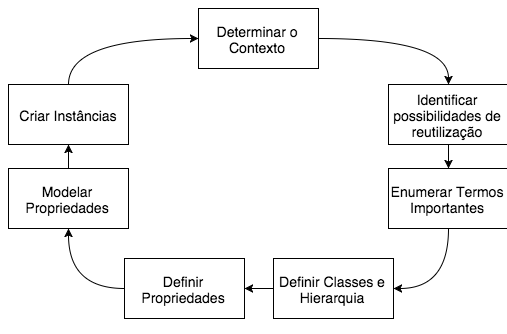
\includegraphics[width=0.7\textwidth]{imagens/desenvolvimento}
	\caption{Processo de desenvolvimento}
	\label{img:desenvolvimento}
\end{figure}

Esta ontologia não tenta definir um processo completo, mas sim propor um conjunto de atividades genéricas que, iterativamente, auxiliarão na representação do contexto trabalho em uma ontologia.

\begin{itemize}
	\item \textbf{Determinar o contexto}: determinar e delimitar o domínio de trabalho, que será representado pela ontologia;
	\item \textbf{Identificar possibilidades de reutilização}: pesquisar por ontologias prontas, fazendo o possível para reutilizar e adaptar trabalhos existentes;
	\item \textbf{Enumerar termos importantes}: listar os termos mais importantes do domínio, os quais devem fazer parte da representação;
	\item \textbf{Definir classes e hierarquia}: transformar a lista de termos importantes em classes, e modelar os relacionamentos entre elas;
	\item \textbf{Definir propriedades}: listar os atributos que devem ser representados para cada uma das classes criadas;
	\item \textbf{Modelar propriedades}: definir como cada um dos atributos listados devem ser representados, e de que forma podem ser reaproveitados;
	\item \textbf{Criar Instâncias}: criar instâncias do mundo real para as classes de representação.
\end{itemize}

	A utilização de tal metodologia neste trabalho deverá, além de ajudar na construção da ontologia, auxiliar na definição e construção do problema. As atividades propostas também serão importantes para a modelagem da solução, já que haverá um intenso estudo do domínio e dos conceitos fundamentais para a sua representação.

% subsection proposta_da_solu_o (end)